\documentclass[12pt]{article}
\usepackage[utf8]{inputenc}
\usepackage{fancyhdr}
\usepackage[includehead, margin=2cm]{geometry}
\usepackage{listings}
\usepackage{titling}
\usepackage{parskip}
\usepackage{fancyvrb}
\usepackage{tabularx}
\usepackage{float}
\usepackage{hyperref}
\usepackage{graphicx}


\usepackage{xcolor}
\lstset{basicstyle=\ttfamily,
  showstringspaces=false,
  commentstyle=\color{red},
  keywordstyle=\color{blue}
}
\newcommand{\codeIn}[1]{{\small\tt{#1}}}
\hypersetup{
    colorlinks=true,
    urlcolor=blue
}

\pagestyle{fancy}

\newenvironment{centeredcode}
{
\ttfamily
\begin{center}
\begin{tabular}{l}
}
{
\end{tabular}
\end{center}
}

\title{CS 4240: Compilers and Interpreters, Project 3, Spring 2023\\
\Large
Assigned: March 27, 2023, 5\% of course grade\\
{Due in Canvas by 11:59pm on April 19, 2023}\\
}
\preauthor{}
\postauthor{}
\author{}
\date{}

\begin{document}
\lhead{CS 4240, Spring 2023}
\rhead{Project 3}
\maketitle
\thispagestyle{fancy}


\section{Project Description}

In this project, you will get familiar with the \href{https://github.com/SVF-tools/SVF/wiki}{SVF} framework, and build a simple reachability analysis tool working on \href{https://llvm.org/docs/LangRef.html#instruction-reference}{LLVM IR}. SVF is a static tool that enables scalable and precise interprocedural dependence analysis on LLVM IRs. Your submitted analysis tool should read the LLVM IR files and decide whether the function call \codeIn{src()} (statically) reaches the function call \codeIn{sink()}. Note that you don't need to analyze flows of values propagated along assignments: simple control-flow path reachability is sufficient.



\subsection{Task Description}
Interprocedural control-flow graph (ICFG)  describes the control flow of the target program. ICFG represents the control instructions from the program entry node to the program exit node and provides multiple control flows among the whole program. The analysis of ICFG can be used to detect the path reachability between two nodes. 

%Source and sink are recognized as the potential nodes for generating and receiving sensitive data in a deceptive program.
Consider the \codeIn{src} and \codeIn{sink} nodes in part of ICFG in Figure~\ref{case1}(a); it is a directed graph with cycles. The red vertex is \codeIn{src} and the blue vertex is \codeIn{sink}. In Figure~\ref{case1}(b), five traversing sequences are provided from \codeIn{src} to \codeIn{sink}. In this project, you will collect all traversing sequences  between two vertices, \codeIn{src} and \codeIn{sink}, while each node in each path of the sequences should only be visited once. Paths containing cycles should
not be collected.

\begin{figure*}[htpb]
    \centering
    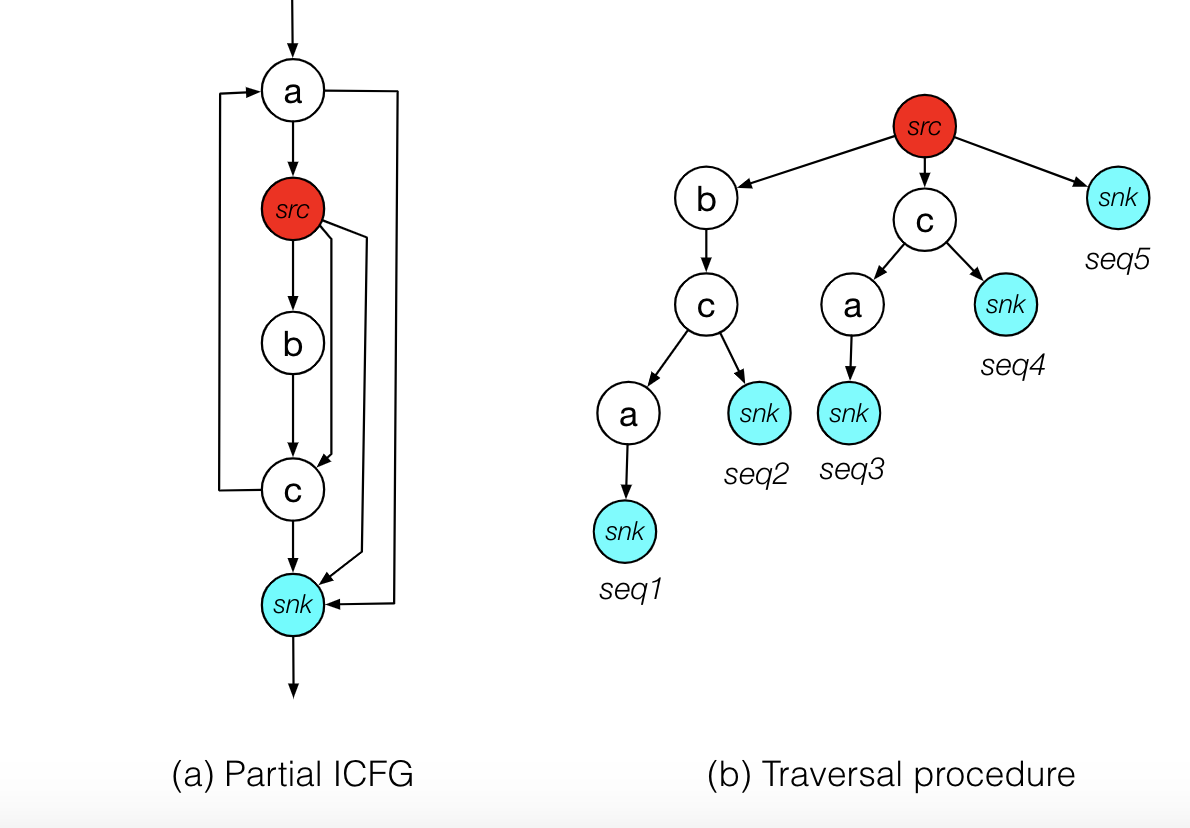
\includegraphics[scale=0.6]{icfgCase1.png}
    \caption{Example}
    \label{case1}
\end{figure*}

You are expected to perform this reachability analysis for
two nodes in each test case. The \codeIn{src} node should be an instruction that contains the \codeIn{src()} function call in the LLVM IR. The \codeIn{sink} node is an instruction that contains the \codeIn{sink()} function call. Your program should
perform the previously mentioned traversals in the ICFG. The ICFG  can be generated by the SVF framework; SVF also provides the functionality to identify instructions represented by the nodes in the ICFG.
One goal in this project is also to learn how to utilize
a real-world static analysis framework to implement analysis
tools. Please start early to get familiar with the SVF framework in this project!
Reference for SVF framework is available at \url{https://github.com/SVF-tools/SVF/wiki}.

\subsection{Project Setup}\label{sec:setup}
To avoid any configuration issues, we will use \href{https://www.docker.com/}{Docker} in this project. We provide a guide to use Docker in your project, and our grading environment will be the same as described in the guide. Here are the instructions to set up, build and test your project.

First you need to install Docker into your local machine. Here is the link to help to get started with Docker: \url{https://www.docker.com/get-started}. If you are a Windows user experiencing installation issues for Docker (rare cases), here we provide some information you may to refer to: \url{https://github.com/SVF-tools/SVF-Teaching/wiki/Windows-docker-installation}.

Once you have Docker installed on your machine, you can pull the provided Docker image from Docker Hub and then work on it. Here is a guide of the entire process on Linux. If you want to know more about Docker please consult the official documentation.

\begin{enumerate}
    \item First you can pull the image from Docker Hub.\\\\
    \codeIn{docker pull cs4240/project3:latest}\\
    \item Then you can start a Docker container from the provided Docker image using the following command.\\\\
    \codeIn{docker run -ti --name=project3-svf-container cs4240/project3:latest /bin/bash}\\\\
    If you want to come back later you can exit the bash session and start the stopped container again using the following command.\\\\
    \codeIn{docker start -ai project3-svf-container}\\\\
    If you want to use VScode dev containers, this command will start the container in the background but will not give you an interactive terminal.\\\\
    \codeIn{docker start project3-svf-container}\\\\
    Select "attach to a running container" from the VSCode extension.
    The docker container named \codeIn{project3-svf-container} will come up. \\
    More info on dev containers can be found \href{https://code.visualstudio.com/docs/devcontainers/containers}{here}. If you're curious you can follow this \href{https://code.visualstudio.com/docs/devcontainers/tutorial}{tutorial} but replace the example container instructions with our docker container.\\\\
    \item To complete this project, you only need to modify the following file inside the container.\\\\
    \codeIn{$\sim$/cs4240\_project3/project3/project3.cpp}\\\\
    After completing the code in this file you can build the project by first going to the directory ``\codeIn{$\sim$/cs4240\_project3/}'' and then running the following command\\\\
    \codeIn{bash build.sh}\\\\
    and test the project by running the following command.\\\\
    \codeIn{bash test.sh}
\end{enumerate}


    
\section{Provided Code}

The only provided code is in the Docker container on Docker Hub, so there is no project directory provided. In the Docker container we have only provided the framework to build the project based on
the dependence of SVF libraries. There will only be a
placeholder \codeIn{project3.cpp} file. In this file, you need to use the SVF framework to generate the ICFG graphs of
the input LLVM IR file. And you need to use SVF to identify the nodes
representing the \codeIn{src()} function call and \codeIn{sink()} function call.
Then your project should perform the reachability analysis and print the result to \codeIn{stdout}.

\section{Grading}
There are in total 100 points for this project.

\subsection{Correct Implementations (60 Points)}

Several test cases are given to you to test the correctness of your project under the \codeIn{$\sim$/cs4240\_project3/tests} directory.

You can run the script \codeIn{test.sh} to check the correctness of your
project for these test cases. If the test script does not show any output, then your project passes the public test cases. There will be hidden test
cases for the project.
For each input test cases, your program is expected to print out the following outputs:
\begin{itemize}
    \item \textbf{First line:} The result whether the \codeIn{src()} function call can reach the \codeIn{sink()} function call (40 Points). If it is reachable, your program should print ``Reachable'', otherwise print  ``Unreachable''. Note that please print the EXACT text of ``Reachable'' or ``Unreachable''. For example, ``UnReachable'' is not an acceptable  output.  If your program provides correct answers to the reachability results, you can get 40 Points.
    \item \textbf{Following lines:} If there are $n$ traveral paths between the \codeIn{src} and \codeIn{sink}, your project should also print $n$ more lines. Each line 
    is a path from \codeIn{src()} to \codeIn{sink()} (20 Points). The path should have
    the following format, supposing that node 1 is the \codeIn{src} node and node 5 is the \codeIn{sink} node: \codeIn{$1-->2-->3-->4-->5$} . If your program provides the \textbf{correct number} of traversal paths between two nodes, you will get the rest 20 Points.
\end{itemize}

\subsection{Performance Evaluation (10 Points)}\label{sec:eval}
If your program can finish running each test case in 30 seconds, you will get 10 Points.

\subsection{Design (30 Points)}\label{sec:design}

In your final report, 
please briefly describe the following:
%
\begin{enumerate}
\item Details about how you generate the ICFG graphs from the input LLVM IR.
\item Details about how you perform the reachability analysis.
\item Any known outstanding bugs or deficiencies that you were unable
  to   resolve before the project submission.
 \end{enumerate}

\section{Submission}\label{sec:sub}
To facilitate the grading, you should not modify
other files in the project directory!
On Canvas, submit a single ZIP file that contains:
\begin{itemize}
    \item The \codeIn{project3.cpp} file
    \item The \codeIn{design.pdf} file described in Section~\ref{sec:design}.
    \item Any test cases you added. (This will not be graded.)
\end{itemize}
\textbf{We will only use the \codeIn{project3.cpp} file to test the correctness of your implementation. If you modify other files, even if your code runs correctly on your local machine,
you will still get points deducted if it cannot run properly in our grading environment.}

\section{Collaboration}
%
We will award identical grades to each member of a given project team,
unless members of the team directly register a formal complaint.
%
We assume that the work submitted by each team is their work solely.
% 
Any clarification question about the project handout should be posted
on the course's public Piazza message
board.
%
Any non-obvious discussion or questions about design and
implementation should be either posted on the course's Piazza message
boards privately for the instructors or presented in person during
office hours.
%
If the instructors determine that parts of the discussion are
appropriate for the entire class, then they will forward selections.
%
Under no condition is it acceptable to use code written by another
team, or obtained from any other source.
%
As part of the standard grading process, each submitted solution will
automatically be checked for similarity with other submitted solutions and with other known
implementations.

\end{document}
